% ******************* PhD Thesis Presentation Template *************************
% Please have a look at the README.md file for info on how to use the template
\PassOptionsToPackage{table}{xcolor} % <-μονο εδω δουλεύει!!

\documentclass[printbib]{Classes/beamerPhD}%%  
% ******************************************************************************
% ******************************* Class Options ********************************
% *********************** See README for more details **************************
% ******************************************************************************
%
% `aspectration=169: reduce ratio to 16:9
%
% `draft': Draft mode images and style option not loaded.(Default draftmode)
%
% `chapter`: This option enables only the specified chapter and it's references
% Useful for review and corrections.
%
% `notes`: Prints frames and notes 
%
% `notes=only`: Prints only notes of each frame
%
% `printbib`: Include bibliography at the end of the presentation 

% ********************************** Preamble **********************************
% Preamble: Contains packages and user-defined commands and settings
% ********************************** Preamble **********************************
% Preamble: Contains packages and user-defined commands and settings
%\usepackage{../sty/beamerthemesimpledso}
%%-----------------------------------------------------------------------------
% % USE THEME
%%-----------------------------------------------------------------------------
\usetheme{simpledso}
% \usetheme{PaloAlto} 
% \usetheme{Singapore}
% \usetheme{Szeged}
% \usetheme{CambridgeUS}
% \usetheme{Montpellier}
% \usetheme{Pittsburgh} <---
% \usetheme{Warsaw}
% \usetheme{Rochester}
% \usetheme{Marburg}
% \usetheme{Malmoe}
% \usetheme{Madrid}
% \usetheme{Luebeck}
% \usetheme{Ilmenau}
% \usetheme{Hannover} <---
% \usetheme{Goettingen}
% \usetheme{Dresden}
% \usetheme{boxes}
% \usetheme{Boadilla}
% \usetheme{Berlin}
% \usetheme{Berkeley}
% \usetheme{AnnArbor}

\usepackage{lmodern}
\usepackage[scale=2]{ccicons}

%%-----------------------------------------------------------------------------
% %  double slides left presentation // right notes NOT WORK WELL!!!
%%-----------------------------------------------------------------------------
% \usepackage{pgfpages}
% \setbeameroption{show notes}
% \setbeameroption{show notes on second screen=right}


%%-----------------------------------------------------------------------------
% %  margins
%%-----------------------------------------------------------------------------
\setbeamersize{text margin left=0.4cm}  % <- like this
\setbeamersize{text margin right=0.4cm} % <- like this
% \setbeamersize{text margin top=0.2cm} % <- like this
% \setbeamersize{text margin bottm=0.2cm} % <- like this

%%-----------------------------------------------------------------------------
% %  SET RATIO TO 16:9 uncoment next line
%%-----------------------------------------------------------------------------
% \usepackage[orientation=landscape,size=custom,width=16,height=9,scale=0.5,debug]{beamerposter} % reduce ratio to 16:9 IUGG defaults!
% Better to use class option!!

%%-----------------------------------------------------------------------------
% % Set background for simpledso theme
%%-----------------------------------------------------------------------------
%\graphicspath{{Chapter3/Figs/Vector/}{Chapter3/Figs/}}
% \setwatermark{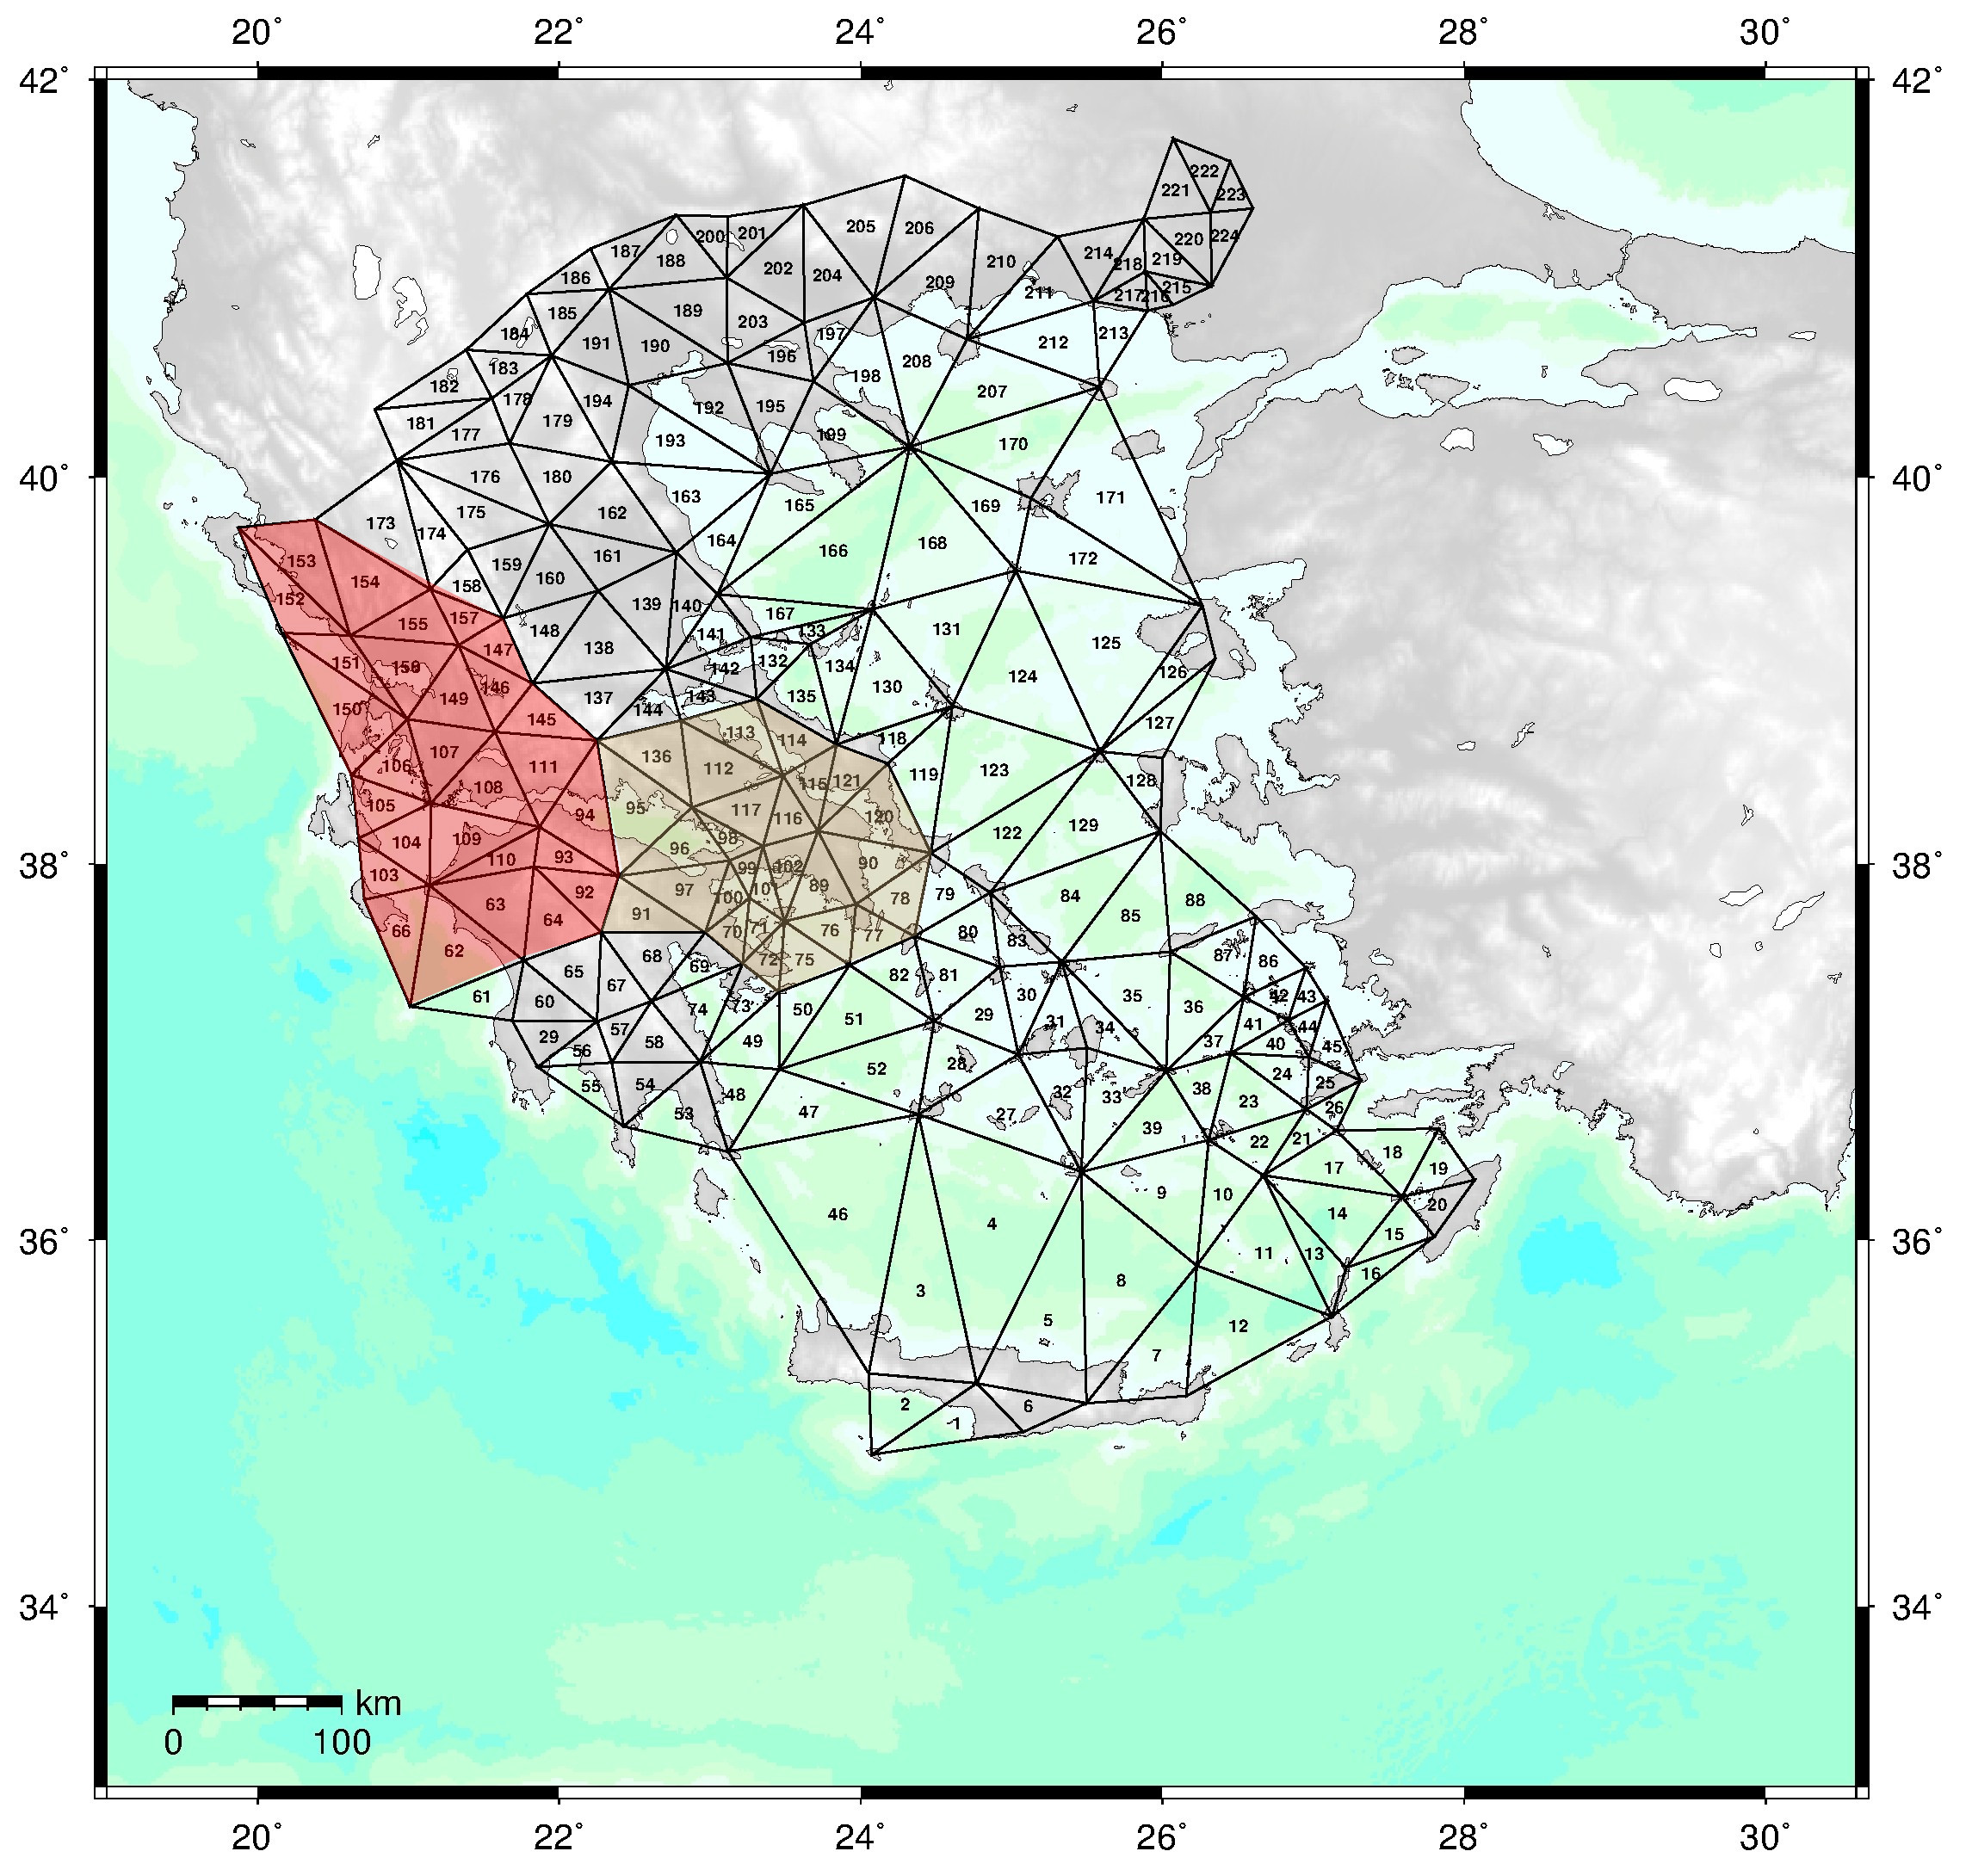
\includegraphics[height=8cm]{Figs/trianglesALL.jpg}}
\setwatermark{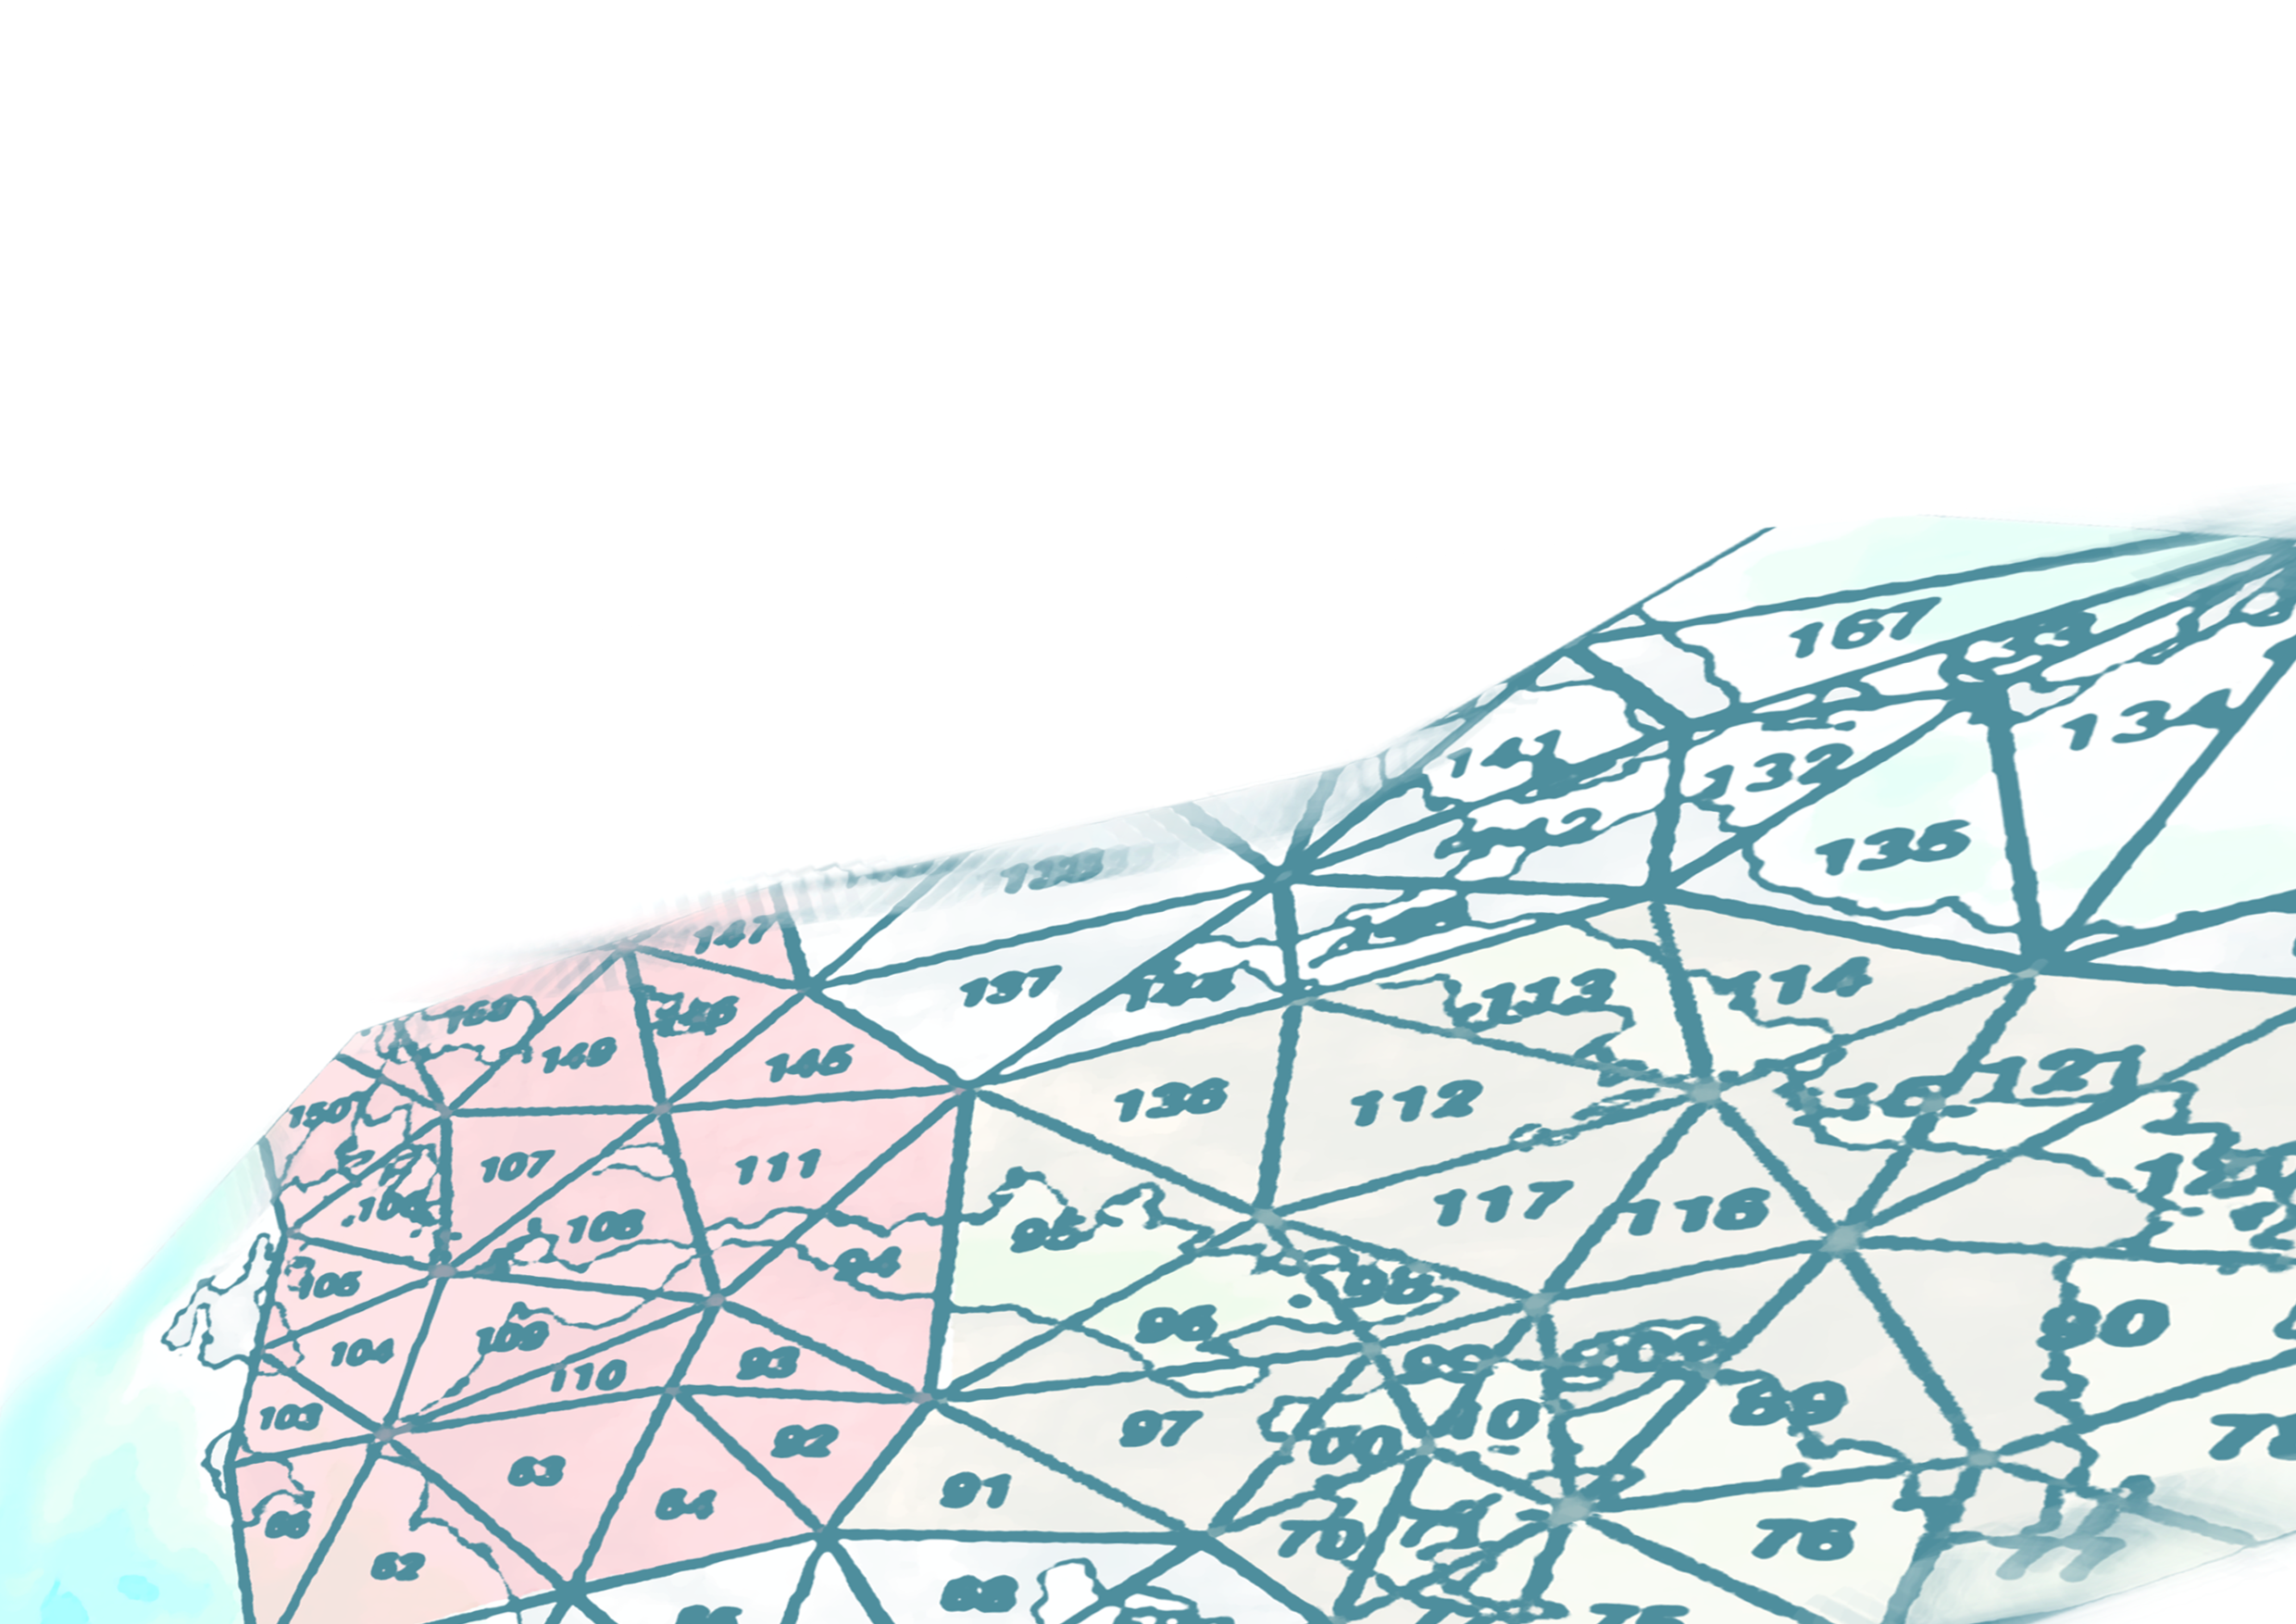
\includegraphics[height=8cm,draft=false]{Figs/backgr01.png}}

%%-----------------------------------------------------------------------------
% Languages
%%-----------------------------------------------------------------------------
% \usepackage[english, greek]{babel}
\usepackage{xgreek}
\usepackage[Greek,Latin]{ucharclasses}
\setTransitionsForGreek{\setlanguage{greek}}{\setlanguage{english}}
% \usepackage{xunicode}
% \usepackage{xltxtra}
% \usepackage[monogreek]{xgreek}
% \usepackage{tabu}

%%-----------------------------------------------------------------------------
% Tables
%%-----------------------------------------------------------------------------
\usepackage{booktabs,tabularx}
\usepackage{tabu}
\usepackage{multirow}

%%-----------------------------------------------------------------------------
% Fonts
%-----------------------------------------------------------------------------
%\usefonttheme{professionalfonts} % using non standard fonts for beamer
%\usefonttheme{serif} % default family is serif
\usepackage{fontspec}
%\setmainfont{Liberation Serif}
% ******************* Fonts (like different typewriter fonts etc.)*************

% Add `customfont' in the document class option to use this section

%\ifsetCustomFont
  % Set your custom font here and use `customfont' in options. Leave empty to
  % load computer modern font (default LaTeX font).
%   \RequirePackage{helvet}

% \setmainfont[Mapping=tex-text]{GFS Didot}
% \setmainfont[Mapping=tex-text]{GFS Bodoni}
% \setmainfont[Mapping=tex-text]{GFS Olga} % είναι λίγο ότι να ναι αυτή!!πλάγια
% \setmainfont[Mapping=tex-text]{GFS Neohellenic}
% \setmainfont[Mapping=tex-text]{GFS Artemisia}
% \setmainfont[Mapping=tex-text]{GFS Elpis} %low resolution printing
% \setmainfont[Mapping=tex-text]{Linux Libertine T}
% \setmainfont[Mapping=tex-text]{Linux Libertine O}

%  % For use with XeLaTeX
%    \setmainfont[
%      Path              = /usr/share/texlive/texmf-dist/fonts/opentype/public/libertine/, %./libertine/opentype/,
%      Extension         = .otf,
%      UprightFont = LinLibertine_R,
%      BoldFont = LinLibertine_RZ, % Linux Libertine O Regular Semibold
%      ItalicFont = LinLibertine_RI,
%      BoldItalicFont = LinLibertine_RZI, % Linux Libertine O Regular Semibold Italic
%    ]
%    {LGR}
%  %  % load font from system font
%     \newfontfamily\libertinesystemfont{Linux Libertine O}
%\fi


% \usepackage{fontspec}
% \setmainfont{TeX Gyre Pagella}
% \setsansfont{TeX Gyre Heros}
% \setmonofont{Inconsolata}
% \setmainfont{Times New Roman}
%\setmainfont{Augie}
 \setsansfont{Arial}
% \setsansfont{Tapir}
% \newfontfamily\greekfont[Script=Greek]{Linux Libertine O}
% \setmainfont{Minion Pro} % substitute with any font that exists on your system
% \setsansfont{Myriad Pro} % substitute with any font that exists on your system
% \setmonofont{Consolas} % substitute with any font that exists on your system
% \usefonttheme[onlymath]{serif}

%%-----------------------------------------------------------------------------
% REQUIRED PACKAGES
%-----------------------------------------------------------------------------
\usepackage{graphicx}  % Required for including images
\usepackage{fancybox}
% \usepackage{xcolor}
%% for tikz
% \usepackage{dtklogos}
\usepackage{tikz}
\usetikzlibrary{mindmap,shadows}
\usepackage{smartdiagram}

% restart numbering footnotes per page
\usepackage{perpage}
\MakePerPage{footnote}
% % Sychronize footnotes on columns minipages
\renewcommand\thempfootnote{\arabic{mpfootnote}}

% use nice itemlists ..
%\usepackage{enumitem, color, amssymb}
\usepackage{url}
% \hypersetup{colorlinks,linkcolor=,urlcolor=links}
\hypersetup{colorlinks=true,allcolors=blue}

% use metalogo to print xelatex!
\usepackage{metalogo}

% % tcolorbox custom block, problem with caption package, cant solve it yet!
% \usepackage[most]{tcolorbox}

%%-----------------------------------------------------------------------------
%% Adgust figures
%%-----------------------------------------------------------------------------
\usepackage{adjustbox} % for \adjincludegraphics
% {\shadowbox{\color{black!35}\includegraphics[height=4cm]{img/iono.eps}}

%%-----------------------------------------------------------------------------
%% Print Arrows
%%-----------------------------------------------------------------------------
\usepackage{marvosym} % \MVRIGHTarrow
\usepackage{stmaryrd} % \shortrightarrow $\Rightarrow$
\usepackage{textcomp} % \textrightarrow

%%-----------------------------------------------------------------------------
%% Math symbols
%%-----------------------------------------------------------------------------
\usepackage{amssymb} 
\usepackage{amsmath}

% \usepackage{soul}
% \definecolor{lightblue}{rgb}{.90,.95,1}
% \sethlcolor{lightblue}
% \renewcommand<>{\hl}[1]{\only#2{\beameroriginal{\hl}}{#1}}
% -----------------------------------------------------------------------------
% CAPTIONS
%-----------------------------------------------------------------------------
\usepackage{caption}
\usepackage{subcaption}
\captionsetup[figure]{font=footnotesize,labelfont=footnotesize,skip=0pt,belowskip=0pt}
\setbeamertemplate{caption}[numbered]

\setbeamerfont{caption}{size=\scriptsize}

% -----------------------------------------------------------------------------
% Four Quad
%-----------------------------------------------------------------------------
\newcommand\FourQuad[4]{
    \begin{minipage}[b][.45\textheight][t]{.50\textwidth}\centering#1\end{minipage}\hfill%
    \begin{minipage}[b][.45\textheight][t]{.50\textwidth}\centering#2\end{minipage}\\[0.1cm]
    \begin{minipage}[b][.45\textheight][t]{.50\textwidth}\centering#3\end{minipage}\hfill
    \begin{minipage}[b][.45\textheight][t]{.50\textwidth}\centering#4\end{minipage}%
}

% -----------------------------------------------------------------------------
% Custom symbols for itemize
%-----------------------------------------------------------------------------

\newenvironment{proenv}{\only{\setbeamercolor{local structure}{fg=green}}}{}
\newenvironment{conenv}{\only{\setbeamercolor{local structure}{fg=red}}}{}
 \usepackage{fontawesome}

% -----------------------------------------------------------------------------
% Rotate text
%-----------------------------------------------------------------------------
\usepackage{rotating}
%\begin{turn}{45} 
% ...
% \end{turn}


% -----------------------------------------------------------------------------
% BIBLATEX
%-----------------------------------------------------------------------------
\usepackage{hyperref}
\usepackage[backend=biber,
            style=authoryear,
            maxbibnames=9,
            maxcitenames=1,
            citestyle=authoryear,
            hyperref=true,
            backref=true,
            sorting=nty,
            natbib=true]{biblatex}

% Hypper linc for all citations use \parencite & \textcite
\ExecuteBibliographyOptions{maxcitenames=1}

\DeclareFieldFormat{citehyperref}{%
  \DeclareFieldAlias{bibhyperref}{noformat}% Avoid nested links
  \bibhyperref{#1}}

\DeclareFieldFormat{textcitehyperref}{%
  \DeclareFieldAlias{bibhyperref}{noformat}% Avoid nested links
  \bibhyperref{%
    #1%
    \ifbool{cbx:parens}
      {\bibcloseparen\global\boolfalse{cbx:parens}}
      {}}}

\savebibmacro{cite}
\savebibmacro{textcite}

\renewbibmacro*{cite}{%
  \printtext[citehyperref]{%
    \restorebibmacro{cite}%
    \usebibmacro{cite}}}

\renewbibmacro*{textcite}{%
  \ifboolexpr{
    ( not test {\iffieldundef{prenote}} and
      test {\ifnumequal{\value{citecount}}{1}} )
    or
    ( not test {\iffieldundef{postnote}} and
      test {\ifnumequal{\value{citecount}}{\value{citetotal}}} )
  }
    {\DeclareFieldAlias{textcitehyperref}{noformat}}
    {}%
  \printtext[textcitehyperref]{%
    \restorebibmacro{textcite}%
    \usebibmacro{textcite}}}



\bibliography{References/triangleref.bib}
\newcounter{bibitmctr}
\newcommand{\brf}{%
  \stepcounter{bibitmctr}%
  \ifnum\value{bibitmctr}=7%
    \setcounter{bibitmctr}{0}
    \framebreak
  \fi
}

\renewbibmacro*{finentry}{\finentry\brf}

% % cahnge fontsize of bibliography for biblatex
\renewcommand*{\bibfont}{\tiny}


% -----------------------------------------------------------------------------
% Insert frame after new section
%-----------------------------------------------------------------------------
% comment next lines if you don't like to use this
\AtBeginSection[]{
  \begin{frame}[b]
%   \vfill
  \vspace{\fill}
  \centering
  \begin{beamercolorbox}[sep=8pt,center,shadow=true,rounded=true]{title}
    \usebeamerfont{title}\Large{\insertsectionhead}%
  \end{beamercolorbox}
  \vskip-2cm
  \begin{flushleft}
    {\color{red!20}\rule{0.7\textwidth}{1pt}}\par
    {\color{red!40}\rule{0.5\textwidth}{1pt}}\par
    {\color{red!60}\rule{0.3\textwidth}{1pt}}\par
    {\color{red!70}\rule{0.16\textwidth}{1pt}}\par
    {\color{red!80}\rule{0.08\textwidth}{1pt}}\par
    {\color{red!90}\rule{0.04\textwidth}{1pt}}\par
  \end{flushleft}
  \vspace{.5cm}
%   \vfill
  \end{frame}
}

% -----------------------------------------------------------------------------
% Configure Draft mode
%-----------------------------------------------------------------------------
% *********************** Configure Draft Mode **********************************
\ifsetDraft
  \usepackage[printwatermark]{xwatermark}
  % Bottom
  \newwatermark*[pages=2-,color=red!60,textalign=center,angle=0,scale=.37,xpos=-.2cm,ypos=-.437\paperheight]{\makebox[.9\textwidth]{{\drafttext}\space-\space{\draftVersion}\space{\timestamp}}}
  %Flush right
%  \newwatermark*[pages=2-,color=red!60,textalign=center,angle=90,scale=.35,xpos=.45\paperwidth, ypos=-.7cm]{\makebox[.9\textwidth]{{\drafttext}\space-\space{\draftVersion}\space{\timestamp}}}
  
\fi 

% Uncomment to disable figures in `draft' mode
% \setkeys{Gin}{draft=true}  % set draft to false to enable figures in `draft'

% These options are active only during the draft mode
% Default text is "Draft"
\SetDraftText{DRAFT}

% Default Watermark location is top. Location (top/bottom)
%\SetDraftWMPosition{bottom}

% Draft Version - default is v1.0
\SetDraftVersion{v1.0}

% Draft Text grayscale value (should be between 0-black and 1-white)
% Default value is 0.75
% \SetDraftGrayScale{0.8}

% Set Draft water mark in print mode. Uncomment next lines
% \usepackage{draftwatermark}
% \SetWatermarkText{\parbox{46cm}{%54 
%   * D R A F T - v0.9.7 * \\ \\
%   * \today * \\ \\
%   compiled via \LaTeX}}
% \SetWatermarkScale{.24}%44
% \SetWatermarkColor[rgb]{1,0,0}


% ******************************** Todo Notes **********************************
%% Uncomment the following lines to have todonotes. % Not working yet!

% \ifsetDraft
%   \usepackage[colorinlistoftodos,prependcaption,textsize=small]{todonotes}
%   \setlength{\marginparwidth}{2.2cm}
% % 	\usepackage[colorinlistoftodos]{todonotes}
% 	\newcommand{\mynote}[1]{\todo[author=mitsos,size=\small,inline,color=green!40]{#1}}
%   \newcommand{\unsure}[1]{\todo[author=mitsos,size=\small,color=red!60]{#1}}
% 	\newcommand{\change}[2][1=]{\todo[author=mitsos,size=\small,linecolor=blue,backgroundcolor=blue!35,bordercolor=blue]{#1}}
% % 	\newcommand{\info}[2][1=]{\todo[linecolor=OliveGreen,backgroundcolor=OliveGreen!25,bordercolor=OliveGreen,#1]{#2}}
% % 	\newcommand{\improvement}[2][1=]{\todo[linecolor=Plum,backgroundcolor=Plum!25,bordercolor=Plum,#1]{#2}}
% 	\newcommand{\xanthos}[1]{\todo[author=xanthos,size=\small,inline,color=red!40]{#1}}
% 	\newcommand{\vagg}[1]{\todo[author=vagg,size=\small,inline,color=red!40]{#1}}
% \else
%   \newcommand{\todo}[1]{}
% 	\newcommand{\mynote}[1]{}
% 	\newcommand{\unsure}[1]{}
% 	\newcommand{\change}[1]{}
% 	\newcommand{\info}[2][1=]{}
% 	\newcommand{\improvement}[2][1=]{}
% 	\newcommand{\xanthos}[1]{}
% 	\newcommand{\vagg}[1]{}
% 	\newcommand{\listoftodos}{}
% \fi
%
% Example todo: \mynote{Hey! I have a note}


% ************************ Thesis Information & Meta-data **********************
% Thesis title and author information, refernce file for biblatex
%% -----------------------------------------------------------------------------
%% PhD section INFO
%% -----------------------------------------------------------------------------
% ************************ Thesis Information & Meta-data **********************
%% The title of the thesis
% \eltitle{ΠΡΟΤΥΠΟ ΠΑΡΟΥΣΙΑΣΗΣ ΣΕ ΠΑΡΙΒΑΛΛΟΝ \\ Beamer-\LaTeX / \XeLaTeX}

%% Subtitle (Optional)
% \subtitle{Using the CUED template}

%% The full name of the author
% \author{ΔΗΜΗΤΡΙΟΥ Γ. ΑΝΑΣΤΑΣΙΟΥ}
\authorname{ΔΗΜΗΤΡΙΟΣ Γ. ΑΝΑΣΤΑΣΙΟΥ}
\authortitle{Διπλ. Αγρονόμος \& Τοπογράφος Μηχανικός Ε.Μ.Π}

%% Department (eg. Department of Engineering, Maths, Physics)
\dept{ΣΧΟΛΗ ΑΓΡΟΝΟΜΩΝ \& ΤΟΠΟΓΡΑΦΩΝ ΜΗΧΑΝΙΚΩΝ}

%% Laboratory
\lab{ΚΕΝΤΡΟ ΔΟΡΥΦΟΡΩΝ ΔΙΟΝΥΣΟΥ}

%% University and Crest
\university{ΕΘΝΙΚΟ ΜΕΤΣΟΒΙΟ ΠΟΛΥΤΕΧΝΕΙΟ}

% Crest minimum should be 30mm.
\crestleft{
\includegraphics[width=\textwidth,draft=false]{Figs/ntua.png}}
\crestright{
\includegraphics[width=0.85\textwidth,draft=false]{Figs/DSOtrans.png}}
%% Use this crest, if you are using the college crest

%% Crest long miminum should be 65mm
%\crest{\includegraphics[width=0.45\textwidth]{University_Crest_Long}}

%% College shield [optional] 
% Crest minimum should be 30mm.
% \collegeshield{\includegraphics[width=0.2\textwidth]{CollegeShields/Kings}}

%% Full title of the Degree
% \degreetitle{ΔΙΔΑΚΤΟΡΙΚΗ ΔΙΑΤΡΙΒΗ}

% Supervisor
% \supervisor{......O/E.........\\ ....Θέση..........}

%% College affiliation (optional)
% \city{ΑΘΗΝΑ}

%% Submission date
% Default is set as {\monthname[\the\month]\space\the\year}
% \degreedate{\today} 
% \degreedate{5 Ιουλίου 2017}

%% Meta information
% \subject{Γεωδαισία} \keywords{{Γεωδαισία} {Τριγωνισμός} {Παραμόρφωση} {Ελλάδα}}

%% Add "thank you" text% 
\thankutext{Ευχαριστώ για την προσοχή σας !}

%% Contact e-informations
\urlin{https://www.linkedin.com/in/demitrisanastasiou/}
\urlgh{https://github.com/demanasta}
\urlgp{https://plus.google.com/u/0/+DemitrisAnastasiou}
\urltw{https://twitter.com/DemAnast}

%% -----------------------------------------------------------------------------
%% Publication's section INFO
%% -----------------------------------------------------------------------------
%% The title of the thesis
\prestitle{Α Beamer-\LaTeX / \XeLaTeX template \\ for conference presentations }

%% The team prepare this presentation
\presteam{
\underline{D.Anastasiou}\textsuperscript{1},
X. Pap.\textsuperscript{2},
V. Zach.\textsuperscript{1},
 A., Mar.\textsuperscript{2}}

%% Organizations of the team
\presorgn{\textsuperscript{1}National Technical University of Athens -- Dionysos Satellite Observatory\\
\textsuperscript{2}School of Rural \& Surveying Engineering -- Laboratory of Higher Geodesy
}

%Contact informations
\presweb{dionysos.survey.ntua.gr}  % webpage
\presmail{dganastasiou@gmail.com}  % contact mail

%% Conference details, Select  text or logo type
% \confname{EUREF Analysis Centre Workshop}
% \confdetail{AIU Bern, Switzerland, October 14-5, 2015}
%% OR conf logo....
\conflogo{
\includegraphics[width=.8\textwidth,draft=false]{Figs/conflogo.png}}






%% -----------------------------------------------------------------------------
%% Course section INFO
%% -----------------------------------------------------------------------------




% ***************************** Chapter Mode ***********************************
% The chapter mode allows user to only print particular chapters with references

\ifdefineChapter
% \includeonly{Chapter1/ch1pres}
\includeonly{Chapter2/ch2pres}
% \includeonly{Chapter3/ch3pres}
% \includeonly{Chapter4/ch4pres}
% \includeonly{Chapter5/ch5pres}
% \includeonly{Chapter6/ch6pres}
% \includeonly{Appendix/ap_refs}
% \includeonly{Appendix/ap_soft}
% \includeonly{Appendix/cut01.tex}
\fi

% ***********************  Start the document  ***********************************
\begin{document}

% *****************************  Make title  *************************************
\maketitle

% *****************************  TOC  *************************************
\begin{frame}
  \frametitle{Δομή Παρουσίασης}
  \tableofcontents
\end{frame}


% ************************  Include Chapters  *************************************
\section{Εισαγωγικά}
 
% \graphicspath{Figs/}

\begin{frame}\frametitle{Λίγα Λόγια...}\framesubtitle{}
Το παρόν πρότυπο αφορά κυρίως παρουσιάσεις διπλωματικών εργασιών, διδακτορικών διατριβών καθώς η αρχική σελίδα είναι διαμορφωμένη ώστε να περιλαμβάνει το τίτλο του πτυχίου, το όνομα του επιβλέποντος κτλ.

Η παρουσίαση διαμορφώθηκε στα Ελληνικά καθώς είναι πιο δύσκολη η διαχείρισή τους στο \LaTeX  αλλά προφανώς μπορεί κάποιος να γράψει στα Αγγλικά. 

Έχουν προστεθεί κάποια slide με βασικές εντολές διαμόρφωσης στο beamer και για να φανεί η δομή της παρουσίασης. Σ

\end{frame}
\note{}

\section{Επιστημονικό Υπόβαρθο}
 
\graphicspath{{Chapter2/Figs/Vector/}{Chapter2/Figs/Raster/}}

%% \subsection{Γενικά}
%\begin{frame}\frametitle{Γεωτεκτονικό υπόβαθρο}
%\label{fr2:gbackground}
%\end{frame}
%\note{}

\section{Μεθοδολογία}

\graphicspath{{Chapter3/Figs/Vector/}}

\begin{frame}
  \frametitle{Εισαγωγή εξισώσεων και εικόνων}
  \framesubtitle{Ανάλυση τριγώνου - Ο αλγόριθμος του Frank}
  \label{fr3:frank_tr}
  \begin{columns}
    \begin{column}{.65\textwidth}
    \vskip.1cm
      {\small Η διαφορά της γωνίας σε δύο χρονικές στιγμές:}
      \[ \delta\phi_\alpha=\delta \theta_\beta - \delta \theta_\gamma \]
 \vskip.1cm
{\small Οι συνιστώσες της διάτμησης:}
  \begin{tiny}
  \begin{align*}
  \gamma_1=\frac{\sin\left ( \theta_\gamma + \theta_\alpha \right )\left ( \delta\phi_\alpha/\sin\alpha_\alpha \right ) - \sin\left ( \theta_\beta + \theta_\gamma \right )\left ( \delta\phi_\beta/\sin\alpha_\beta \right )}{\sin\phi_\gamma} \\
  \gamma_2=\frac{\cos\left ( \theta_\gamma + \theta_\alpha \right )\left ( \delta\phi_\alpha/\sin\alpha_\alpha \right ) - \cos\left ( \theta_\beta + \theta_\gamma \right )\left ( \delta\phi_\beta/\sin\alpha_\beta \right )}{\sin\phi_\gamma}
  \end{align*}
  \end{tiny}
   {\small Η τιμή της ολικής διάτμησης και το αζιμούθιο των κύριων αξόνων της έλλειψης της ανηγμένης παραμόρφωσης:}
    \end{column}
    \begin{column}{.34\textwidth}
      \centering
          \adjincludegraphics[width=.98\linewidth, valign=t]{FrankTR.jpg}
          
          {\tiny \parencite{Frank1966}}
    \end{column}
  \end{columns}
\vskip-.5cm  
\begin{columns}
  \begin{column}{.3\textwidth}
    \begin{small}
  \vskip-1cm
      \begin{equation*}
        E=\begin{bmatrix}
        \varepsilon_{11} & \varepsilon_{12}\\ 
        \varepsilon_{21} & \varepsilon_{22}
        \end{bmatrix}
      \end{equation*}
    \end{small}
  \end{column}
  \begin{column}{.03\textwidth}
    \vskip-1cm
    \textbf{$\Rightarrow$}
  \end{column}
  \begin{column}{.3\textwidth}
    \begin{scriptsize}
      \begin{align*}
        \gamma _1=\varepsilon_{11} - \varepsilon_{22}, \\
        \gamma _2=\varepsilon_{12} + \varepsilon_{21}, \\ 
        \omega = \frac{1}{2} \left (\varepsilon_{12} - \varepsilon_{21}  \right )\\
      \end{align*}
    \end{scriptsize}
  \end{column}
   \begin{column}{.03\textwidth}
     \vskip-1cm
    \textbf{$\Rightarrow$}
  \end{column}
  \begin{column}{.3\textwidth}
  
%   \begin{tcolorbox}[height=1.5cm, width=2.5cm]
%     \begin{scriptsize}
%       \begin{align*} 
%         \gamma = \sqrt{{\gamma_{1}}^{2}+{\gamma_{2}}^{2}}\\
%         \tan 2\psi = \frac{\gamma_1}{\gamma_2} \\
%       \end{align*}
%     \end{scriptsize}
%     \end{tcolorbox}
    
% \begin{varblock}[2.5cm]{}
  \centering
    \begin{scriptsize}
      \begin{align*} 
        \gamma = \sqrt{{\gamma_{1}}^{2}+{\gamma_{2}}^{2}}\\
        \tan 2\psi = \frac{\gamma_1}{\gamma_2} \\
      \end{align*}
    \end{scriptsize}
% \end{varblock}
  \end{column}
\end{columns}


\end{frame}
\note{} % Add notes for this slide
\section{Δεδομένα}

\graphicspath{{Chapter4/Figs/Vector/}}

\begin{frame}
  \frametitle{Χρήση του Πακέτου 'tikz'}
  \framesubtitle{Προφανώς οι φωτογραφίες είναι από τα Τζουμέρκα!!}
  \label{fr4:hist_pics}
  
  \begin{tikzpicture}
    \node (img1) {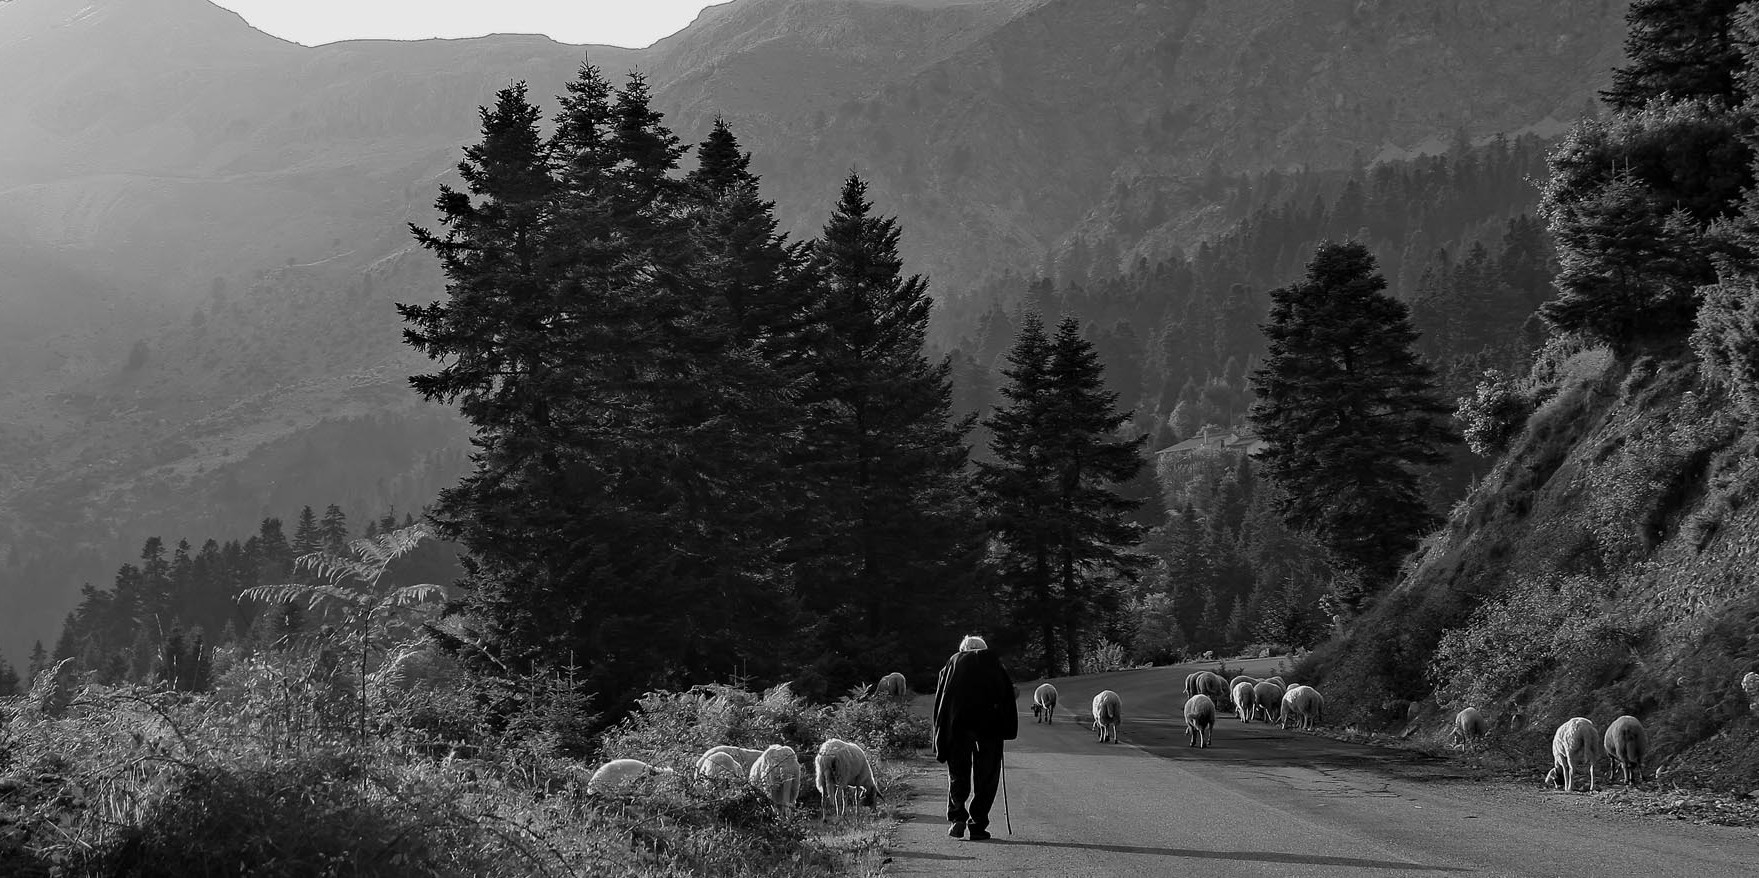
\includegraphics[height=3.6cm]{tsopanos.jpg}};
    \node (img2) at (img1.south west) [yshift=-1.2cm, xshift=.5cm]{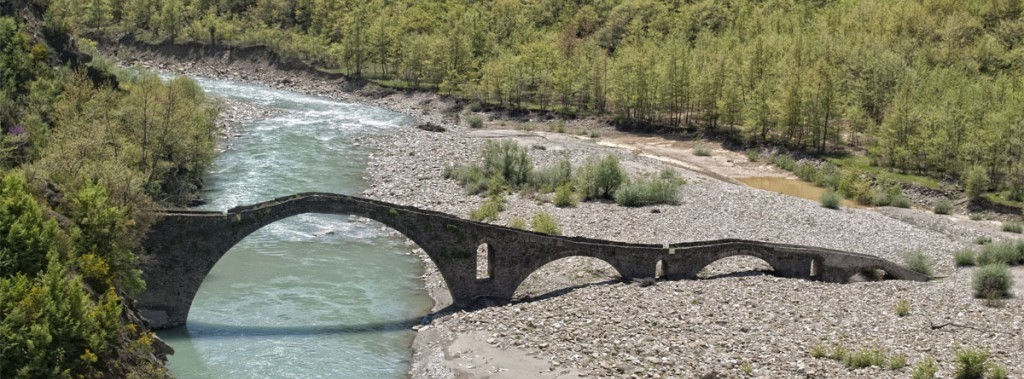
\includegraphics[height=3cm]{br-papastathi.jpg}};
    \node (img3) at (img2.north west) [yshift=1.7cm, xshift=1.5cm] {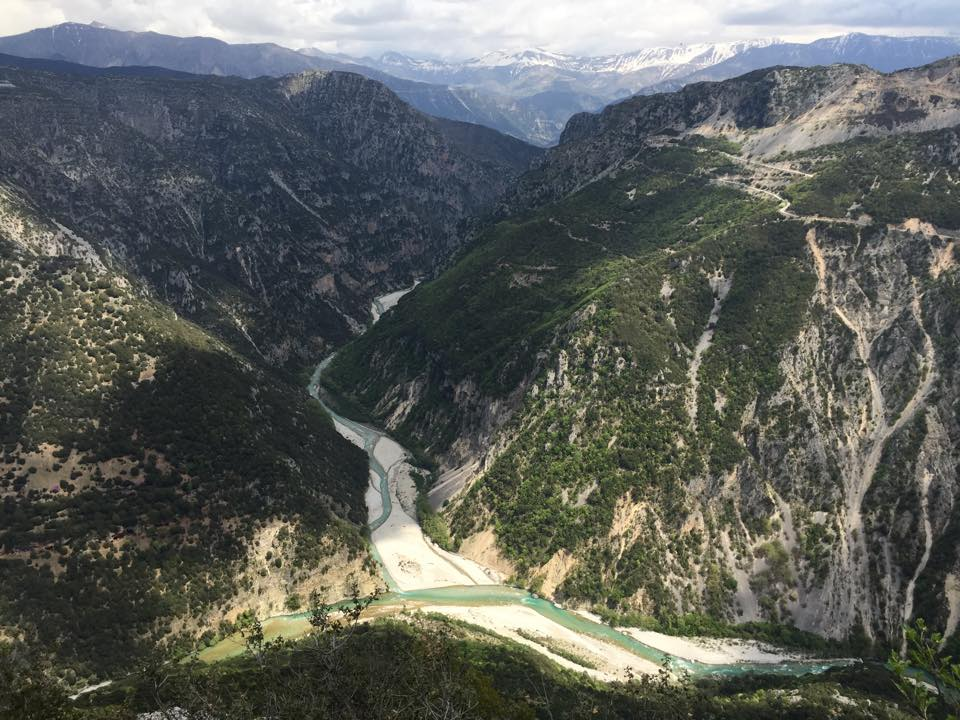
\includegraphics[height=3.2cm]{smiksi.jpg}};
    \node (img4) at (img2.east) [yshift=-.8cm,xshift=1.2cm] {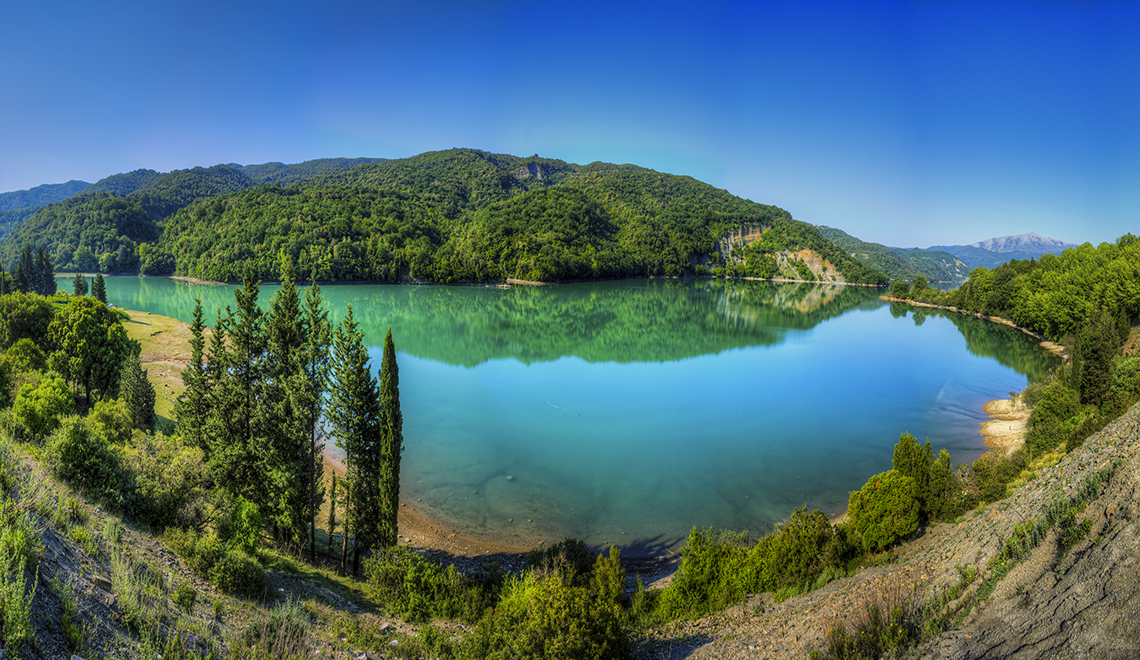
\includegraphics[height=1.8cm]{rouista.jpg}};
  \end{tikzpicture}
  

\end{frame}
\note{}

\section{Επεξεργασία \& Ανάλυση}

\graphicspath{{Chapter5/Figs/Vector/}{Chapter4/Figs/Vector/}}

\begin{frame}
  \frametitle{Χρήση animation στο ίδιο Slide}
  \framesubtitle{}
  \label{fr6:terr_sat_ext}
  \begin{columns}
    \begin{column}{.5\textwidth}
      \underline{Έμφαση σε συγκεκριμένη πρόταση:}
      \begin{itemize}
        \item<1>  Πρόταση 1 .618
        \item<2>  Πρόταση 2 .718
        \item<3-> Πρόταση 3 .141 
      \end{itemize}
      
 
    \end{column}
    \begin{column}{.5\textwidth}
    \underline{Έμφαση με τη σειρά εμφάνισης:}
     \begin{itemize}
        \item<1-> Πρόταση 1 .6180339887
        \item<2-> Πρόταση 2 .7182818284
        \item<3-> Πρόταση 3 .1415926535
      \end{itemize}
    \end{column}
  \end{columns}
  
  \begin{center}
    \vskip .5cm
    \underline{Κάθε κείμενο υπερκαλύπτει το προηγούμενο:} \\
    \vskip .5cm
    \begin{overprint}\centering
      \onslide<3-> {Εμφανίζεται μόνο στη Πρόταση 3} \\
      \onslide<1> Πρόταση 1 .61803398874989484820...
      \onslide<2> Πρόταση 2 .718281828459045235360287471352...
      \onslide<3-> Πρόταση 3 .14159265358979323846264338327950288419716939937510...
    \end{overprint}
  \end{center}
\end{frame}
\note{}
\section{Συμπεράσματα}

% \graphicspath{{Chapter8/Figs/Vector/}}

%\begin{frame}
%  \frametitle{Συμπεράσματα}
%  \framesubtitle{}
%  \label{fr8:concl1}

%\end{frame}
%\note{}

% % \section{Δημοσιεύσεις  - Λογισμικό}

\begin{frame}
  \frametitle{Δημοσιευμένες εργασίες}
  \framesubtitle{}

  
\begin{scriptsize}
    \begin{itemize}
\item[\faFile] Anastasiou D., Chouliaras G., Papanikolaou X., Marinou A., Zacharis V., Galanis J., Drakatos G., Paradissis D. (2015) \textbf{Geodetic and seismological analysis of the January 26, 2014 Cephalonia Island earthquake sequence.}  \textit{26th General Assembly of the IUGG,Prague, Czech Republic, 22/6 - 2/7.}\\
  \item[\faFile] Ganas A., Marinou A., Anastasiou D., Paradissis D., Papazissi K., Tzavaras P. and Drakatos G. (2013). \textbf{GPS-derived estimates of crustal deformation in the central and North Ionian Sea, Greece: 3-yr results from NOANET continuous network data.} \textit{Journal of Geodynamics 67, Pages 62–71A, DOI:\url{10.1016/j.jog.2012.05.010}}\\
    \item[\faFile] Papazissi K., Anastasiou D., Marinou A., Mitsakaki C., Papanikolaou X., Paradissis D. (2010) \textbf{Deformation studies in the Gulf of Patras, Western Greece.} \textit{Honorary Volume in honor of D.Arabelo, Professor of the Aristotle University of Thessaloniki.}\\
    \item[\faFile] Anastasiou D., Marinou A., Mitsakaki C., Papazissi K., Papanikolaou X., Paradissis D. (2010). \textbf{Crustal Deformation in the Patras Gulf, Greece, from GPS Data Analysis.} \textit{15th General Assembly of Wegener, Istanbul, Turkey, 14 – 17 September.}\\
  \end{itemize}
  \end{scriptsize}

\end{frame}

% % \section{Συμπεράσματα}

\begin{frame}
  \frametitle{Ρουτίνες λογισμικού}
  \framesubtitle{}
\underline{\textbf{Αποθετήριο OS code}: \href{https://github.com/demanasta}{https://github.com/demanasta \faGithub}}
\vskip.2cm
\begin{footnotesize}
Το λογισμικό έχει αναπτυχθεί στα πλαίσια της διδακτορικής διατριβής και των ερευνητικών δραστηριοτήτων του Κέντρου Δορυφόρων Διονύσου και του Εργαστηρίου Ανώτερης Γεωδαισίας και διατίθεται υπό την άδεια GPL-v3.0 ως ελεύθερο λογισμικό/λογισμικό ανοιχτού κώδικα (ΕΛ/ΛΑΚ).
\vskip.3cm
\begin{tabular}{l p{9cm}}
\textbf{1. GeoToolbox:} & Ρουτίνες σε περιβάλλον Matlab για την ανάλυση των τεκτονικών ταχυτήτων και των υπολογισμό τανυστών ανηγμένης παραμόρφωσης (\href{http://demanasta.github.io/GeoToolbox/}{http://demanasta.github.io/GeoToolbox/}) \\
\textbf{2. gpsvel:} & Σχεδιασμός χαρτών τεκτονικών ταχυτήτων και τανυστών ανηγμένης παραμόρφωσης σε περιβάλλον GMT (\href{http://demanasta.github.io/gpsvel/}{http://demanasta.github.io/gpsvel/}) \\
\textbf{3. plot\_eq:} & Σχεδιασμός χαρτών καταλόγων σεισμών στην περιοχή της Ελλάδας (\href{http://demanasta.github.io/plot\_eq/}{http://demanasta.github.io/plot\_eq/}) \\
\textbf{4. GNSS\_nets:} & Σχεδιασμός χαρτών απεικόνισης δικτύων GNSS και αποτελεσμάτων της επεξεργασίας σε περιβάλλον GMT (\href{http://demanasta.github.io/GNSS\_nets/}{http://demanasta.github.io/GNSS\_nets/}) \\
\end{tabular}
\end{footnotesize}
\end{frame}


%%-----------------------------------------------------------------------------
%% END OF PRESENTATION ...
%%-----------------------------------------------------------------------------

% ************************  Thank you frame  **********************************
% include Thank U last frame
\makethanku % Ιncluded to class file

% ************************  Bibliography  *************************************
% % % Add 'printbib' option in Class file to Include Bibliography
\ifdefinePrintbib
  \begin{frame}[t,allowframebreaks]
    \frametitle{Βιβλιογραφία}
    \printbibliography
  \end{frame}
\fi

% ************************  Cut Frames  **************************************
% Add back up cut frames
% % \section{Κομμένα}

\graphicspath{{Chapter2/Figs/Vector/}{Chapter2/Figs/Raster/}{Chapter3/Figs/Vector/}{Chapter4/Figs/Vector/}{Chapter5/Figs/Vector/}{Chapter6/Figs/Vector1/}{Chapter7/Figs/Vector/}{Chapter8/Figs/Vector/}}

% ----------------------------------------------------------------------------
% % CHAPTER 2
%-----------------------------------------------------------------------------

\begin{frame}
  \frametitle{Πρόσφατες εργασίες για την περιοχή}
  \label{fr2:previousIonio}
\begin{columns}
  \begin{column}{.49\textwidth}
  \begin{block}{\textcite{Chousianitis2015}}
  \begin{footnotesize}
    Βόρειo Ιόνιο: Επιμήκυνση Β-Ν.\\
    Κεντρικό: Περιστροφική Κίνηση 6-8$^{\circ}$/My.\\
    Νότιο: Επιμήκυνση ΔΝΔ-ΑΒΑ.\\
    Κορινθιακός: Επιμήκυνση Β-Ν.
  \end{footnotesize}
  \end{block}
  \centering
    \includegraphics[width=.8\linewidth]{chousian2015.png}
%     {\tiny \parencite{Chousianitis2015}}
  \end{column}
  \begin{column}{.49\textwidth}
  \begin{block}{\textcite{Perouse2013}}
\begin{footnotesize}
  Κεντρικό Ιόνιο ως ξεχωριστό μπλοκ.\\
  Διερεύνηση των ορίων στη Δυτική πλευρά.
  \end{footnotesize}
  \end{block}
  \centering
    \includegraphics[width=.8\linewidth]{perouseZones344.png}
%     {\tiny \parencite{Perouse2013}}
  \end{column}
\end{columns}

\end{frame}
\note{}


\begin{frame}
  \frametitle{Υπάρχουσες εργασίες}
  \framesubtitle{Σεισμολογικά Δεδομένα}
  \label{fr2:pr_seism}
    \begin{block}{\textcite{Papazachos1971}}%<1->
    Ερμηνεία των τεκτονικών και γεωφυσικών χαρακτηριστικών του Ελληνικού τόξου.
    \end{block}
    \begin{block}{\textcite{McKenzie1972}}%<2->
    Προτείνονται 2 μικροπλάκες, του Νοτίου Αιγαίου και της Κεντρικής-Βορείου Ελλάδος.
    \end{block}
    \begin{block}{\textcite{LePichon1979}}%<3>
    Επιλύσεις των μηχανισμών γένεσης για την εκτίμηση του πεδίου παραμόρφωσης της Ανατολικής
    Μεσογείου.
    \end{block}
    % \footfullcite{Papazachos1971}
    % \footfullcite{Drewes1982}
\end{frame}
\note{}

\begin{frame}
  \frametitle{Υπάρχουσες εργασίες}
  \framesubtitle{Γεωδαιτικά Δεδομένα}
  \label{fr2:pr_geod}
    \begin{block}{\textcite{Drewes1982}}
    Δεδομένα 20 γεωδαιτικών σταθμών παρατήρησης με την τεχνική SLR.\par
    Εκτίμηση της περιστροφικής κίνησης των δύο μικροπλακών στην Ανατολική Μεσόγειο
    \end{block}
\vskip-.2cm
    \begin{block}{\textcite{Billiris1991}}
    Μετρήσεις του τριγωνομετρικού δικτύου 1\textsuperscript{ης} τάξης των περιόδων 1890, 1980.\par
    Σχετική μετατόπιση στον Κορινθιακό Κόλπο από 40 έως 60 cm.\par
    Νοτιοδυτική κίνηση της Πελοποννήσου σε σχέση με τη Βόρεια Ελλάδα.
    \end{block}
\vskip-.2cm
    \begin{block}{\textcite{stiros1993283}}
    38 τριγωνομετρικά σημεία στην Κεντρική Ελλάδα, κοινά σε τρεις διαφορετικές περιόδους\par
    Aριστερόστροφη διάτμηση και διαστολή σε διεύθυνση Β - Ν στον Κορινθιακό Κόλπο μετά το 1930
    \end{block}
\end{frame}
\note{}

\begin{frame}
  \frametitle{Υπάρχουσες εργασίες}
  \framesubtitle{Γεωδαιτικά Δεδομένα}
  \label{fr2:pr_geod2}
\begin{columns}
  \begin{column}{.49\textwidth}
    \begin{block}{\textcite{Veis1992}}
    75 κοινά σημεία των τριγωνισμών \par περιόδων 1890-1982.\par
    Η περιοχή μελέτης διαιρέθηκε σε 9 μπλοκ ομοιογενούς παραμόρφωσης.
    \end{block}
    
    \begin{block}{\textcite{Davies199724571}}
    36 σημεία, επαναμέτρηση με GPS, το 1992.\par
    Σταθμοί SLR Διόνυσος \& Χρυσοκελλαριά\par
    Μετρήσεις σε 10 έκκεντρα.
    \end{block}
  \end{column}
  \begin{column}{.49\textwidth}
  \centering
    \includegraphics[width=.7\linewidth]{veis92_9bl.jpg}

    \includegraphics[width=.7\linewidth]{davies97_tr.png}

  \end{column}
\end{columns}
\end{frame}
\note{}

\begin{frame}
  \frametitle{Υπάρχουσες εργασίες}
  \framesubtitle{Γεωδαιτικά Δορυφορικά Δεδομένα}
  \label{fr2:pr_satgeod2}
  \vskip-.2cm
\begin{columns}[t]
  \begin{column}{.48\textwidth}
    \begin{block}{\textcite{Nyst2004}}
    375 σταθμοί GPS\par
    4 μικροπλάκες\par
%     \begin{itemize}
%       \item Κεντρική Ελλάδα\\
%       \item Νότιο-Κεντρικό Αιγαίο\\
%       \item Ανατολία\\
%       \item Νότιος Μαρμαράς\\
%     \end{itemize}
    \end{block}
    \centering
    \includegraphics[width=.91\linewidth]{nyst04_4bl.png}
  \end{column}
  \begin{column}{.48\textwidth}
    
\begin{block}{\textcite{Reilinger2006}}
440 σταθμοί GPS\par
8 μικροπλάκες
\end{block}
    \centering
    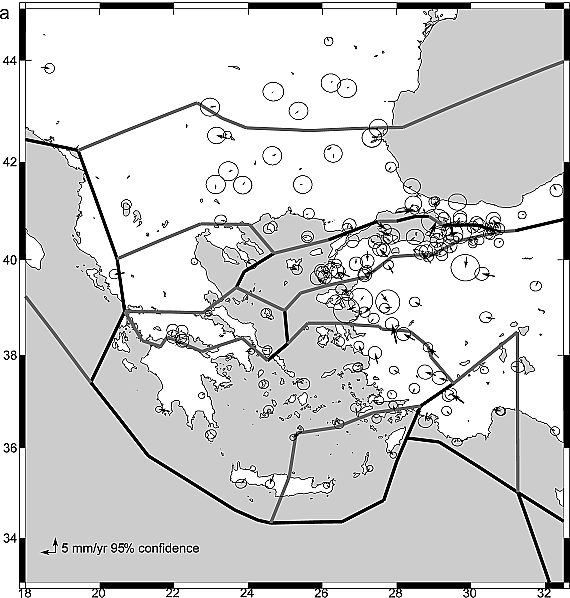
\includegraphics[width=.84\linewidth]{reilinger06_8bl.png}
  \end{column}
\end{columns}
\end{frame}
\note{}

\begin{frame}
  \frametitle{Υπάρχουσες εργασίες}
  \framesubtitle{Γεωδαιτικά Δορυφορικά Δεδομένα}
  \label{fr2:satgeod3}
\begin{columns}
  \begin{column}{.48\textwidth}
    \begin{block}{\textcite{Taymaz1991,Floyd2010}}
    254 σταθμοί GPS\par
    10 μικρομπλόκ
    \end{block}
    \centering  
    \includegraphics[width=.92\linewidth]{floyd10_10bl.png}
  \end{column}
  \begin{column}{.48\textwidth}
    \begin{block}{\textcite{Floyd2010}}
    254 σταθμοί GPS\par
    15 μικρομπλόκ
    \end{block}
    \vskip .4cm
    \centering  
    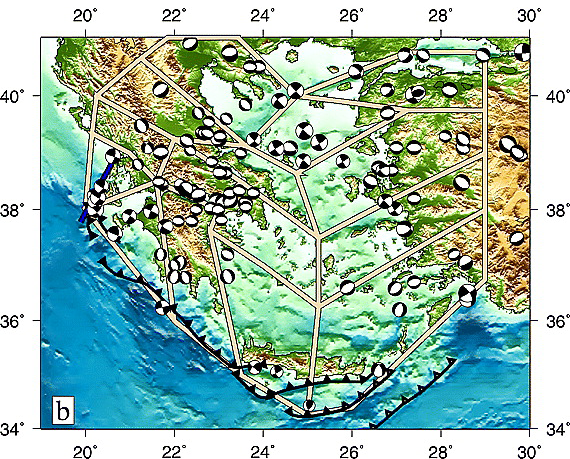
\includegraphics[width=.92\linewidth]{floyd10_15bl.png}
  \end{column}
\end{columns}
% \footfullcite{Floyd2010}
\end{frame}
\note{}



% ----------------------------------------------------------------------------
% % CHAPTER 3
%-----------------------------------------------------------------------------
\begin{frame}
  \frametitle{Αλγόριθμος Frank}
  \framesubtitle{}
  \label{fr3:frank}
  Προϋποθέτει επαναλαμβανόμενες μετρήσεις που έχουν πραγματοποιηθεί στις κορυφές ενός τριγωνομετρικού δικτύου οριζόντιου ελέγχου.
  \begin{equation*}
  \label{eq:velgrad22}
    E=\begin{bmatrix}
    \varepsilon_{11} & \varepsilon_{12}\\ 
    \varepsilon_{21} & \varepsilon_{22}
    \end{bmatrix}
  \end{equation*}
  
  Οι διατμητικές συνιστώσες της ανηγμένης παραμόρφωσης και η περιστροφή:\\
  \[    \gamma _1=\varepsilon_{11} - \varepsilon_{22}, 
  \hspace{.7cm}
      \gamma _2=\varepsilon_{12} + \varepsilon_{21}, 
  \hspace{.7cm}
      \omega = \frac{1}{2} \left (\varepsilon_{12} - \varepsilon_{21}  \right )\]
  
  Η τιμή της ολικής διάτμησης και το αζιμούθιο των κύριων αξόνων της έλλειψης της ανηγμένης παραμόρφωσης:
  \[ \gamma = \sqrt{{\gamma_{1}}^{2}+{\gamma_{2}}^{2}}
  \hspace{1cm}
  \tan 2\psi = \frac{\gamma_1}{\gamma_2} \]


\end{frame}
\note{}

\begin{frame}
  \frametitle{Αλγόριθμος Frank}
  \framesubtitle{Ανάλυση στο τρίγωνο}
  \label{fr3:frank_tr}
  \begin{columns}
    \begin{column}{.65\textwidth}
      Η διαφορά της γωνίας σε δύο χρονικές στιγμές:
      \[ \delta\phi_\alpha=\delta \theta_\beta - \delta \theta_\gamma \]
      
      Θεωρείται ότι η παραμόρφωση είναι ομοιόμορφη σε όλη τη περιοχή του τριγώνου.
      \begin{scriptsize}
      \begin{align*}
\delta\phi_\alpha = \frac{1}{2}\left ( \sin2\theta_\beta - \sin2\theta_\gamma \right )\gamma_1 + \left ( \cos2\theta_\beta - \cos2\theta_\gamma \right )\gamma_2 \\
\delta\phi_\beta = \frac{1}{2}\left ( \sin2\theta_\gamma - \sin2\theta_\alpha \right )\gamma_1 + \left ( \cos2\theta_\gamma -\cos2\theta_\alpha \right )\gamma_2
\end{align*}
      \end{scriptsize}

    \end{column}
    \begin{column}{.34\textwidth}
      \centering
          \adjincludegraphics[width=.98\linewidth, valign=t]{FrankTR.jpg}
          
          {\tiny \parencite{Frank1966}}
    \end{column}
  \end{columns}

  \begin{footnotesize}
  \begin{align*}
  \gamma_1=\frac{\sin\left ( \theta_\gamma + \theta_\alpha \right )\left ( \delta\phi_\alpha/\sin\alpha_\alpha \right ) - \sin\left ( \theta_\beta + \theta_\gamma \right )\left ( \delta\phi_\beta/\sin\alpha_\beta \right )}{\sin\phi_\gamma} \\
  \gamma_2=\frac{\cos\left ( \theta_\gamma + \theta_\alpha \right )\left ( \delta\phi_\alpha/\sin\alpha_\alpha \right ) - \cos\left ( \theta_\beta + \theta_\gamma \right )\left ( \delta\phi_\beta/\sin\alpha_\beta \right )}{\sin\phi_\gamma}
  \end{align*}
  \end{footnotesize}

\end{frame}
\note{}

% ----------------------------------------------------------------------------
% % CHAPTER 4
%-----------------------------------------------------------------------------


% ----------------------------------------------------------------------------
% % CHAPTER 5
%-----------------------------------------------------------------------------
\begin{frame}
  \frametitle{Διαχρονική Ανάλυση}
  \framesubtitle{Η περιοχή της Δυτικής Ελλάδας}
  \label{fr5:allpp_ionio}
  \begin{columns}
    \begin{column}{.5\textwidth}
    \centering
      \textcolor{red}{\small Άξονες επιμήκυνσης}\\
      \includegraphics[width=\linewidth]{ext_ionio.jpg}

    \end{column}
    \begin{column}{.5\textwidth}
    \centering
      \textcolor{blue}{\small Ολική διάτμηση ($\dot{\gamma}_{tot}$)}\\
      \includegraphics[width=\linewidth]{shear_ionio.jpg}

    \end{column}
  \end{columns}
\end{frame}
\note{}


% ----------------------------------------------------------------------------
% % CHAPTER 6
%-----------------------------------------------------------------------------
\begin{frame}
  \frametitle{Επίγεια \& Δορυφορικά Γεωδαιτικά Δεδομένα}
  \framesubtitle{}
  \label{fr6:terr_sat_ext}
  \begin{columns}
    \begin{column}{.5\textwidth}
     \centering
     {\footnotesize  Άξονες επιμήκυνσης,\\ επίγειες παρατηρήσεις}\\
      \includegraphics[width=.9\linewidth]{ext_ionio.jpg}

    \end{column}
    \begin{column}{.5\textwidth}
    \centering
    {\footnotesize  Κύριοι άξονες ($\dot{e}_{max}$, $\dot{e}_{min}$).}\\
      \includegraphics[width=\linewidth]{ciontrSTR.jpg}

    \end{column}
  \end{columns}
\end{frame}
\note{}

\begin{frame}
  \frametitle{Περιοχή Κεντρικού Ιονίου -Πατραϊκού Κόλπου}
  \framesubtitle{Μοντέλο 5 μπλοκς}
  \label{fr6:str_5bl}
  \vskip.1cm
  \begin{columns}
    \begin{column}{.5\textwidth}
    \centering
    {\footnotesize  Κύριοι άξονες ($\dot{e}_{max}$, $\dot{e}_{min}$).}\\
      \includegraphics[width=\linewidth]{ptr05bSTR.jpg}

    \end{column}
    \begin{column}{.5\textwidth}
    \centering
      {\footnotesize  Ρυθμός περιστροφής ($\dot{\Omega}$).}\\
      \includegraphics[width=\linewidth]{ptr05bROT.jpg}

    \end{column}
  \end{columns}
  \vskip-.1cm
  \begin{table}[H]{\tiny
     \begin{center}
      \begin{tabular*}{\linewidth}{@{\extracolsep{\fill}}c c c c c c}
\toprule
% \multicolumn{1}{r}{} &\multicolumn{5}{c}{blocks} \\
% \cline{2-6}
\multicolumn{1}{r}{} &1 & 2 & 3 & 4 & 5\\
\midrule
%  φ  & 38.185 & 38.607 & 38.317 & 37.907 & 38.385 \\
%  λ  & 21.019 & 21.726 & 21.996 & 21.731 & 21.617 \\
 $\dot{e}_{max}$ $\pm$ σ$_{\dot{e}_{max}}$  &  +0.058 $\pm$ 0.027 & +0.050 $\pm$ 0.051 & +0.411 $\pm$ 0.083 & +0.011 $\pm$ 0.045 & +0.293 $\pm$ 0.073 \\
 $\dot{e}_{min}$ $\pm$ σ$_{\dot{e}_{min}}$  &  -0.104 $\pm$ 0.029 & -0.032 $\pm$ 0.038 & -0.098 $\pm$ 0.112 & -0.050 $\pm$ 0.050 & -0.087 $\pm$  0.089\\
 Az$_{\dot{e}_{max}}$ $\pm$ σ$_{Az_{\dot{e}_{max}}}$ & -11.185 $\pm$  6.041 & 25.962 $\pm$ 23.816 & 13.949  $\pm$  6.932 & 16.187 $\pm$ 28.914 & 12.255 $\pm$  7.544\\
 $\dot{\Omega}$  $\pm$ σ$_{\dot{\Omega}}$ & +7.439 $\pm$ 0.973 & +3.605 $\pm$  1.946 & -0.401 $\pm$ 3.548 & +2.976 $\pm$ 1.774 & +6.294 $\pm$  2.861 \\
 $\dot{\gamma}_{tot}$ $\pm$ σ$_{\dot{\gamma}_{tot}}$ & 0.162 $\pm$ 0.040 & 0.082 $\pm$ 0.064 & 0.509 $\pm$ 0.140 & 0.061 $\pm$ 0.068 & 0.380 $\pm$  0.115 \\
\bottomrule
\multicolumn{6}{l}{φ, λ, Az$_{\dot{e}_{max}}$ in deg; $\dot{e}_{max}$, $\dot{e}_{min}$, $\dot{\gamma}_{tot}$ in μstrain/y ;  $\dot{\Omega}$ in deg/My }
   \end{tabular*}
 \end{center}}
\end{table}
\end{frame}
\note{}


% ----------------------------------------------------------------------------
% % CHAPTER 7
%-----------------------------------------------------------------------------


% ----------------------------------------------------------------------------
% % CHAPTER 8
%-----------------------------------------------------------------------------

\begin{frame}
  \frametitle{Συμπεράσματα}
  \framesubtitle{Εκτίμηση επιφανειακών παραμορφώσεων}
  \label{fr8:concl2}
  \begin{itemize}
    \item 1η π.α.: Ολική διάτμηση της τάξης των 80 nstrain/y.\\
    \item 2η - 3η π.α.: Αύξηση των τιμών ολικής διάτμησης.\\
%     \item Διαφορές στο πεδίο παραμόρφωσης πριν και μετά το 1930 στον σε Πατραϊκό Κορινθιακό Κόλπο.\\
  \end{itemize}
  \textbf{Δυτική Ελλάδα:}
  \begin{itemize}
    \item Αλλαγή στο πεδίο παραμόρφωσης πριν και μετά το 1930.\\
    \item Πατραϊκός-Κορινθιακός: Αλλαγή στη διεύθυνση της ολικής διάτμησης σε ΑΝΑ - ΔΒΔ, παράλληλα στη διεύθυνση των ρηγμάτων.\\
    \item Επιμήκυνση της περιοχής σε διεύθυνση Β - Ν.\\
  \end{itemize}
  \textbf{Ανατολική Στερεά:}
  \begin{itemize}
    \item Επανιδρύθηκαν πολλά τριγωνομετρικά σημεία.\\
    \item Επιμήκυνση της περιοχής στη διεύθυνση ΒΑ - ΝΔ \parencite{Veis1992,Davies199724571}.\\
    \item 3η π.α, Καπαρέλλι-Ερυθρές: Επιμήκυνση ΒΒΔ - ΝΝΑ.\\
    Δεν συμφωνεί με τη γενική κινηματική εικόνα της περιοχής, συμφωνεί με \textcite{Marinou2015a}. \\
  \end{itemize}
\end{frame}
\note{}












% *********************** end of document ************************************
\end{document}
